%% A simple template for a term report using the Hagenberg setup
%% based on the standard LaTeX 'report' class

%%% Magic comments for setting the correct parameters in compatible IDEs
% !TeX encoding = utf8
% !TeX program = pdflatex 
% !TeX spellcheck = en_US
% !BIB program = biber

\RequirePackage[utf8]{inputenc} % Remove when using lualatex or xelatex!
\RequirePackage{hgbpdfa}				% Remove if NO PDF/A output is desired

\documentclass[language=english,titlepage=false,smartquotes=true]{hgbreport}
% Supported options in [..]:
%    Main language: language=english (default), language=german
%    Typographic quotes: smartquotes=true, smartquotes=false (default)
%    APA citation style: apa=true, apa=false (default)
%    Title page: titlepage=true (default), titlepage=false
%    Page layout: twoside=false (single-sided, default), twoside=true (double-sided)
%    Update check: updatecheck=true (default), updatecheck=false (to suppress)
%%%-----------------------------------------------------------------------------

\graphicspath{{images/}}  % Location of images and graphics
\bibliography{hgbreferences} % Biblatex bibliography file (hgbreferences.bib)

%%%-----------------------------------------------------------------------------
\begin{document}
%%%-----------------------------------------------------------------------------

\author{Simone B.\ Feldbacher, Andreas \ Schrattenecker}                    % Your name
\title{VCO2IL Computer Vision\\ % Name of the course or project
			Term Report}	                 % or "Project Report"
\date{\today}

%%%-----------------------------------------------------------------------------
\maketitle
%%%-----------------------------------------------------------------------------

\begin{abstract}\noindent



\bigskip
\noindent
Use the abstract to provide a short summary of the document's contents.
\end{abstract}

%%%-----------------------------------------------------------------------------
\tableofcontents
%%%-----------------------------------------------------------------------------

\part{Class Exercises}
\chapter{Exercise 1}
\begin{comment}
\section{Goal}
The objective of this exercise was to investigate several classical computer vision techniques using thermal and RGB images captured by a drone. The exercise focused on panorama stitching, feature matching across different image modalities, camera calibration, and estimation of the drone's relative motion. In addition to implementing the algorithms, their performance and limitations were evaluated on the provided datasets.

\section{Procedure}
Describe the procedure here.

\section{Results}
Summarize results.
\end{comment}

\section{Introduction}

This chapter summarizes the implementation and evaluation of several computer vision algorithms using the drone image datasets provided. The implemented methods include panorama stitching, feature matching, camera calibration, and extrinsic pose estimation.


\section{Panorama Stitching}

Panorama stitching was performed using OpenCV's built-in \texttt{Stitcher} class. The implementation is shown in Program~\ref{prog:stitch} and Program~\ref{prog:stitch_thermal}.

\begin{program}[H]
\caption{Panorama stitching using OpenCV}
\label{prog:stitch}
\begin{verbatim}
stitcher = cv2.Stitcher_create()

_, panorama = stitcher.stitch(images["RGB"])

imshow(panorama)
\end{verbatim}
\end{program}

\begin{figure}[H]
    \centering
    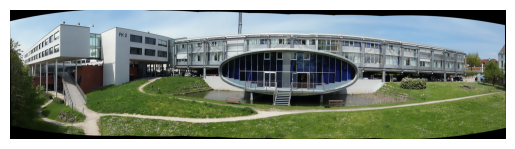
\includegraphics[width=\textwidth]{images/panorama_rgb.png}
    \caption{Panorama generated from the RGB images.}
\end{figure}

\begin{program}[H]
\caption{Thermal panorama stitching}
\label{prog:stitch_thermal}
\begin{verbatim}
_, panorama = stitcher.stitch(images["Thermal"])

imshow(panorama)
\end{verbatim}
\end{program}

\begin{figure}[H]
    \centering
    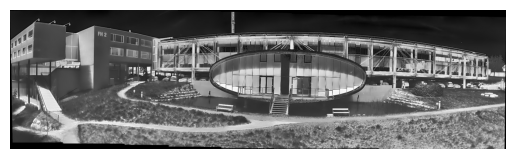
\includegraphics[width=\textwidth]{images/panorama_thermal.png}
    \caption{Panorama generated from the thermal images.}
\end{figure}

The panorama was successfully generated for both the RGB and thermal image sets. The resulting panoramas show that the provided image sequence contains sufficient overlap for automatic image alignment.


\section{Feature Matching}

To compare feature descriptors for thermal and RGB images, SIFT, ORB, and AKAZE were evaluated on all four provided datasets. The features were detected independently in both images, matched using a brute-force matcher, and filtered using the Lowe ratio test. The number of detected keypoints and the remaining good matches were recorded for each descriptor.

\begin{program}[H]
\caption{Feature detection and matching}
\label{prog:feature_matching}
\begin{verbatim}
thermal = cv2.cvtColor(images["Thermal"][0], cv2.COLOR_BGR2GRAY)
rgb = cv2.cvtColor(images["RGB"][0], cv2.COLOR_BGR2GRAY)

kp_t, des_t = detector.detectAndCompute(thermal, None)
kp_r, des_r = detector.detectAndCompute(rgb, None)

bf = cv2.BFMatcher(norm_type)
matches = bf.knnMatch(des_t, des_r, k=2)

good_matches = []
for m, n in matches:
    if m.distance < 0.75 * n.distance:
        good_matches.append(m)
\end{verbatim}
\end{program}

The same procedure was applied to all four scenes using the SIFT, ORB, and AKAZE descriptors. The resulting number of key points detected and good matches is summarized in Table~\ref{tab:feature_matching}.

\begin{table}[H]
    \centering
    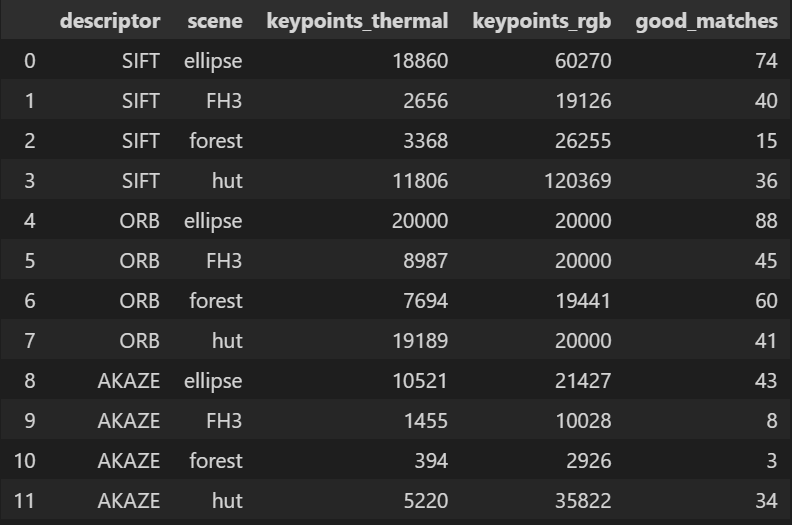
\includegraphics[width=0.8\textwidth]{images/feature_matching.png}
    \caption{Comparison of feature descriptors on the four datasets.}
    \label{tab:feature_matching}
\end{table}

ORB and SIFT produced the most useful results. ORB generated the highest number of good matches after increasing the maximum number of detected features, while SIFT provided stable results with fewer features. AKAZE produced fewer correspondences in all scenes. The quality of the matches should be evaluated not only by the number of matches, but also by the ratio of good matches and by geometric verification using RANSAC inliers.

\section{Camera Calibration}

Camera calibration was performed using the provided chessboard images, as the scene images are not suitable for intrinsic calibration. Chessboard corners were detected and refined before estimating the intrinsic camera parameters and distortion coefficients with OpenCV's calibration functions. To determine the influence of the number of calibration images, the calibration was repeated with an increasing number of images.

\begin{program}[H]
\caption{Camera calibration using chessboard images}
\label{prog:calibration}
\begin{verbatim}
found, corners = cv2.findChessboardCorners(gray, chessboard_size)

if found:
    corners = cv2.cornerSubPix(
        gray, corners, (11,11), (-1,-1), criteria
    )

    object_points.append(objp)
    image_points.append(corners)

error, K, dist, _, _ = cv2.calibrateCamera(
    object_points,
    image_points,
    gray.shape[::-1],
    None,
    None,
)
\end{verbatim}
\end{program}

\begin{program}[H]
\caption{Evaluation of the required number of calibration images}
\label{prog:calibration_evaluation}
\begin{verbatim}
for i in range(2, len(calibration_images) // 2 + 1):
    error, _, _, _, _ = calibrate(calibration_images[:i])
    print(f"Reprojection error with {i} images: {error:.4f} pixels")
\end{verbatim}
\end{program}

\begin{figure}[H]
    \centering
    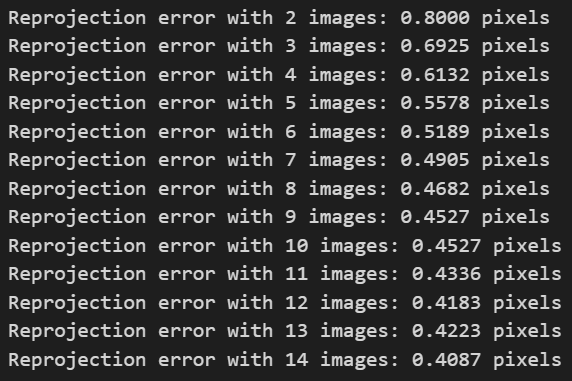
\includegraphics[width=0.8\textwidth]{images/reprojection_error.png}
    \caption{Reprojection error for an increasing number of calibration images.}
    \label{fig:calibration_output}
\end{figure}

Calibration was successful using the provided chessboard images. As shown in Figure~\ref{fig:calibration_output}, at least three images were required to obtain a reliable calibration. Increasing the number of images reduced the reprojection error from 0.6925 pixels to 0.4087 pixels, while the improvement became smaller with additional images.


\section{Extrinsic Estimation}

The relative camera pose was estimated from two consecutive RGB images. SIFT was used to detect and match feature points. The essential matrix was computed using \texttt{findEssentialMat()}, and the relative rotation and translation direction were recovered with \texttt{recoverPose()}. The provided intrinsic camera calibration was used for pose estimation.

\begin{program}[H]
\caption{Relative pose estimation}
\label{prog:pose_estimation}
\begin{verbatim}
sift = cv2.SIFT_create()

kp1, des1 = sift.detectAndCompute(gray1, None)
kp2, des2 = sift.detectAndCompute(gray2, None)

matches = cv2.BFMatcher().knnMatch(des1, des2, k=2)

good_matches = []
for m, n in matches:
    if m.distance < 0.75 * n.distance:
        good_matches.append(m)

E, _ = cv2.findEssentialMat(pts1, pts2, K)

_, R, t, _ = cv2.recoverPose(E, pts1, pts2, K)
\end{verbatim}
\end{program}

\begin{figure}[H]
    \centering
    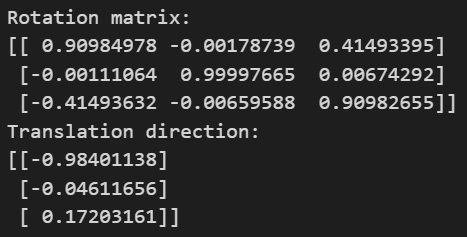
\includegraphics[width=0.60\textwidth]{images/camera_calibration.png}
    \caption{Estimated rotation matrix and translation direction.}
    \label{fig:extrinsic_output}
\end{figure}

The relative rotation and translation direction were successfully estimated. The quality of the estimation depends on the accuracy of the feature matches and can be evaluated using the number of RANSAC inliers.


\section{Conclusion}

The implemented computer vision methods were successfully applied to the drone datasets provided. RGB panorama stitching produced reliable results, while feature matching showed that SIFT and ORB provided the most suitable descriptors for thermal-to-RGB matching. Camera calibration was successfully performed using chessboard images, achieving a low reprojection error. Finally, the relative camera pose was estimated using feature correspondences and the essential matrix.
\chapter{Exercise 2}

\section{Introduction}

This exercise investigates different approaches for image compression. The main focus is on compression of the frequency domain using the Discrete Cosine Transform (DCT), where the effect of removing frequency coefficients on image quality and compression ratio is analyzed.

Additionally, Implicit Neural Representations (INRs) are discussed as an alternative approach for image representation and compression.


\section{Frequency Domain Compression}

\subsection{Implementation}

The DCT compression algorithm was implemented using OpenCV. The main steps are shown below:

\begin{program}[H]
\caption{DCT image compression}
\label{prog:dct_compression}
\begin{verbatim}
def dct_compress(image, keep_ratio=0.25):
    gray = cv2.cvtColor(image, cv2.COLOR_RGB2GRAY).astype(np.float32)
    dct = cv2.dct(gray)

    h, w = dct.shape
    keep_h = int(h * np.sqrt(keep_ratio))
    keep_w = int(w * np.sqrt(keep_ratio))

    compressed = np.zeros_like(dct)
    compressed[:keep_h, :keep_w] = dct[:keep_h, :keep_w]

    reconstructed = cv2.idct(compressed)
    reconstructed = np.clip(reconstructed,0,255).astype(np.uint8)

    return reconstructed, compressed
\end{verbatim}
\end{program}

The function first converts the RGB image to grayscale and applies the DCT. Compression is achieved by keeping only the low-frequency coefficients in the upper-left part of the DCT matrix. The remaining coefficients are discarded by setting them to zero. Finally, the inverse DCT reconstructs the compressed image.
The effect of this compression process is illustrated in Figure~\ref{fig:dct_example}.


\subsection{Results and Analysis}

The quality of reconstruction was first evaluated using a fixed value $\texttt{keep\_ratio}$ of 25\%. Figure~\ref{fig:dct_example} shows the original grayscale image, the reconstructed image after DCT compression, and the retained DCT coefficients.

\begin{figure}[H]
    \centering
    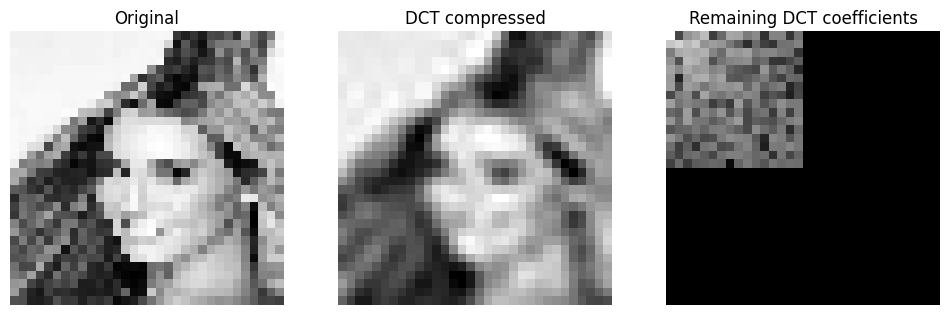
\includegraphics[width=\textwidth]{dct_example.png}
    \caption{Comparison between the original image, the DCT compressed reconstruction using $\texttt{keep\_ratio}=0.25$, and the retained DCT coefficients.}
    \label{fig:dct_example}
\end{figure}

The reconstructed image preserves the main structure of the face, while some high-frequency details are removed due to the discarded coefficients. This shows that the low-frequency components contain important information for reconstructing the overall appearance of the image.

To further analyze the influence of compression strength, different values of $\texttt{keep\_ratio}$ were tested (5\%, 10\%, 25\%, 50\% and 75\%). The reconstructed images and their corresponding MSE values are shown in Figure~\ref{fig:dct_ratios}.

\begin{figure}[H]
    \centering
    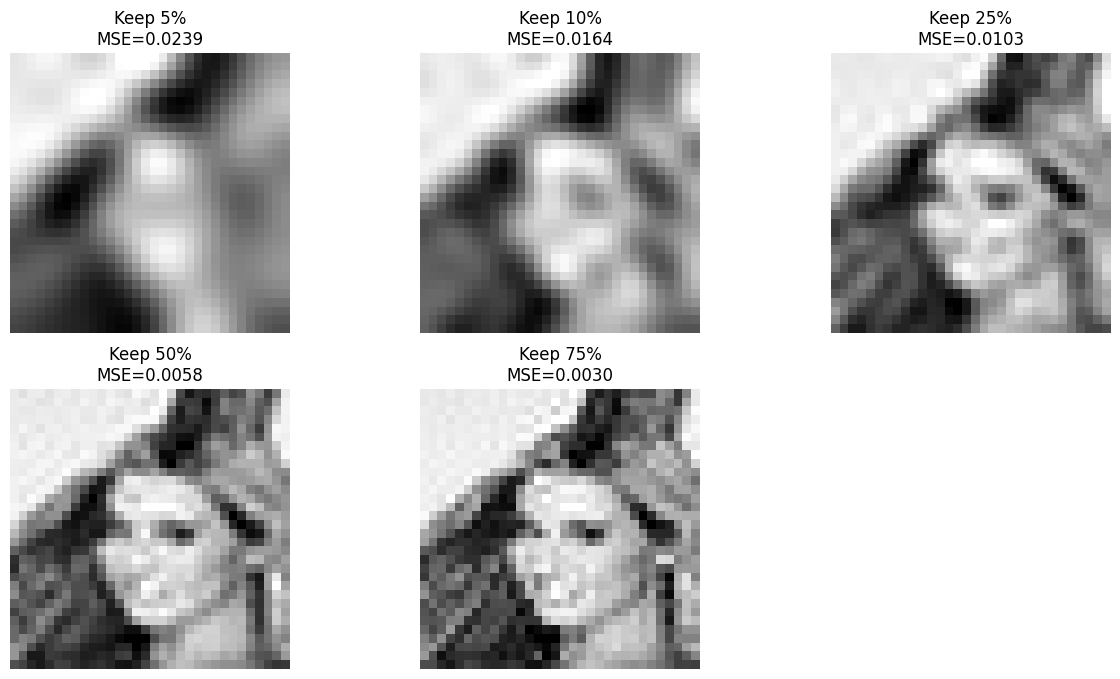
\includegraphics[width=\textwidth]{dct_ratios.png}
    \caption{Reconstructed images for different $\texttt{keep\_ratio}$ values. Lower values result in stronger compression and higher reconstruction error.}
    \label{fig:dct_ratios}
\end{figure}

Removing more DCT coefficients increases compression, but reduces reconstruction quality. Lower $\texttt{keep\_ratio}$ values lead to a more visible loss of detail, blurrier images, and higher MSE values. Higher values preserve more information and result in better visual quality, but provide less compression. A medium $\texttt{keep\_ratio}$ provides a good balance between compression and reconstruction quality.

The theoretical compression ratio depends on the number of retained DCT coefficients. For example, keeping only 5\% of the coefficients results in approximately a 20:1 compression ratio, while keeping 50\% results in 2:1 compression. Therefore, $\texttt{keep\_ratio}$ provides direct control over the trade-off between storage reduction and image quality.


\section{Implicit Neural Representations}

\subsection{Concept}

Implicit Neural Representations (INRs) represent images using neural networks instead of directly storing pixel values. The network learns a function that maps the coordinates of the image $(x,y)$ to the RGB values. The network parameters are then used as the image representation.

The size of the network influences the trade-off between compression and reconstruction quality. Larger networks can represent more details and improve reconstruction quality, but require more parameters and therefore more storage. Smaller networks provide stronger compression, but may lose image details.

The number of training epochs also affects the quality of reconstruction. More epochs usually improve the result, but increase the required computation time. Positional encoding helps INRs capture high-frequency details such as edges and textures, resulting in sharper reconstructions.

\subsection{Comparison}

Compared to frequency-domain methods, INRs use a neural network representation instead of storing frequency coefficients. DCT-based compression is usually faster because reconstruction only requires mathematical transformations, while INRs require the evaluation of the neural network.

INRs can represent fine details more flexibly, especially when positional encoding is used. However, this flexibility comes with higher computational costs. Frequency-domain methods are simpler and faster, but removing high-frequency coefficients can lead to loss of image details.


\section{Conclusion}

This exercise investigated image compression using frequency-domain methods and implicit neural representations.

DCT-based compression showed that reducing the number of frequency coefficients can significantly decrease the required storage while preserving the main structure of the image. The parameter $\texttt{keep\_ratio}$ provides direct control over the trade-off between compression ratio and reconstruction quality. However, removing too many coefficients leads to increased MSE and loss of image details.

INRs provide a different approach by representing images through neural network parameters instead of frequency coefficients. They can capture complex details, especially when using positional encoding, but require higher computational effort for training and reconstruction.

Overall, both approaches involve a trade-off between compression efficiency and image quality. DCT offers a simple and fast compression method, while INRs provide a more flexible representation with increased computational requirements.


\part{Related Work Research - Real time Hand Gesture Recognition}
\chapter{Introduction}
Introduce the research topic and scope.

\chapter{Hand Tracking}
 
\section{Overview}
Gesture recognition is a central part of human-computer interaction. It allows hand movements to be used directly as input signals. Computer-vision-based approaches are particularly popular, since they need no special sensors and work with cameras that are already widely available. This makes them well suited for real applications such as virtual and augmented reality, sign language recognition, and general user interfaces \cite{qiComputerVisionbasedHand2024, cuiDeepVisionbasedRealtime2025}. A remaining problem is that recognition often becomes unreliable under changing lighting, cluttered backgrounds, or partial occlusion \cite{qiComputerVisionbasedHand2024}.
 
Gesture recognition systems are usually split into two groups: vision-based and sensor-based approaches. Sensor-based methods, such as data gloves, electromyography, or inertial measurement units, give signals that barely depend on the environment, but they need extra hardware and are less convenient to use. Vision-based methods instead work contactless and feel more natural, but they are more sensitive to lighting, background, and occlusion \cite{qiComputerVisionbasedHand2024, shinMethodologicalStructuralReview2024}. Since both approaches have different strengths and weaknesses, they are increasingly combined instead of being seen as competitors \cite{wangComprehensiveSurveyMultimodal2026}.
 
\section{Vision-Based Recognition}
 
\subsection{Processing Pipeline}
Vision-based systems usually follow the same basic pipeline: data acquisition, preprocessing to reduce noise and lighting variation, segmentation of the hand region, feature extraction, and finally classification \cite{qiComputerVisionbasedHand2024}. Segmentation is especially important, since mistakes here carry over into every following step and lower the overall performance.
 
For feature extraction, both classic descriptors (Histogram of Oriented Gradients, Local Binary Patterns, geometric contour features) and learned deep features are used. Learned features tend to adapt better across different datasets. For classification, Support Vector Machines and Hidden Markov Models used to be the standard but have mostly been replaced by neural networks \cite{qiComputerVisionbasedHand2024}.
 
RGB-D cameras like Microsoft Kinect or Intel RealSense add depth information to this pipeline, which helps with segmentation and makes the system more robust against lighting changes and cluttered backgrounds. Real-time performance, sensor accuracy, and generalization to new environments are still open problems \cite{qiComputerVisionbasedHand2024}.
 
\subsection{From Hand-Crafted Features to Deep Learning}
Early systems relied on manually defined features and did not generalize well outside controlled settings. Deep learning changed this by extracting features automatically from raw data. Convolutional Neural Networks are good at capturing spatial structure, while Long Short-Term Memory networks were initially used to model how gestures change over time \cite{cuiDeepVisionbasedRealtime2025}. More recently, transformer and attention-based models have started to replace recurrent networks, since they can model long-range dependencies and put more weight on relevant image regions, which improves performance on more complex gestures \cite{shinMethodologicalStructuralReview2024}.
 
\section{Sensor-Based Recognition}
Surface electromyography (sEMG) is one of the main sensor-based alternatives to vision. It measures electrical muscle activity to figure out which gesture was performed. Since it does not depend on visual conditions, it is useful for applications like prosthetic control or wearable interfaces. Deep learning models can now work directly on raw sEMG signals, so manual feature engineering is no longer necessary. The main problem that remains is that muscle signals vary a lot between individuals, which makes it hard to build models that generalize across users \cite{zanghieriSEMGbasedHandGesture2023}.
 
\section{Multimodal Fusion}
To work around the limits of a single modality, more research combines RGB, depth, skeletal, and sEMG data into multimodal systems. The main benefit is robustness: if one sensor fails, for example vision under occlusion, another modality such as an inertial or muscle-based sensor can compensate \cite{wangComprehensiveSurveyMultimodal2026}. The main difficulty is that these data sources are very different from each other in resolution, noise, and information content, which makes fusion non-trivial \cite{shinMethodologicalStructuralReview2024}.
 
To fuse this data, hybrid deep-learning architectures are commonly used, combining CNNs for spatial features with recurrent or graph networks for temporal and structural dependencies. Transformers are increasingly used as well, since they can flexibly integrate different data sources \cite{wangComprehensiveSurveyMultimodal2026}. Mahmud et al. show this in practice by combining depth and skeletal data for dynamic gesture recognition, reporting clear improvements over single-modality baselines, especially for gestures that look visually similar \cite{mahmudDeepLearningbasedMultimodal2024}.
 
\section{Open Challenges}
Across vision-based, sensor-based, and multimodal systems, deep learning is now the common foundation, and the general trend is moving from single-modality pipelines toward multimodal fusion for better robustness. Challenges that keep showing up across the literature are the lack of standardized, realistic benchmarks, limited real-time capability, and poor generalization to new users and environments \cite{shinMethodologicalStructuralReview2024, wangComprehensiveSurveyMultimodal2026}.


\chapter{Common Aspects of Signed Languages}
Discuss common aspects, literature summary, definitions.

\chapter{Conclusion and Outlook}

This report has provided an overview of the current state of research in the field of hand gesture recognition and highlighted some of its applications in sign language translation. Examining the relevant literature revealed a trend towards deep learning-based approaches, which have yielded significant improvements in accuracy and robustness. Another common theme in both chapters was the use of multimodal data to make up for the limitations of a single video feed. Supplementary depth maps and skeletal data can make up for ambiguity caused by lighting and occlusion in the image. 


Foregoing the gloss representation stage in sign translation has shown both promising results in accuracy as well as reduced the work required in creating suitable training data. For deep learning-based approaches, the availability of large, annotated datasets is crucial. The covered literature focuses on American and German sign language, which have a large number of speakers and thus a larger pool of data. Enabling translation of less popular sign languages, specific regional dialects and individual signing styles, requires a lower barrier for data collection and annotation. 

Automated sign recognition and production has the potential to improve accessibility online and in real life. In education, new tools could be developed to complement traditional teaching methods, which would allow for wider adoption of the language. It is, however, important to note that sign language is traditionally taught by non-hearing individuals in an effort to preserve the culture and history of a language that has been historically marginalized \cite{ASLTeachingEthics}. Besides the technical challenges, the social and cultural implications of who gets to build and control these systems will become increasingly important as the technology matures.
%%%-----------------------------------------------------------------------------
\appendix                                                   % Switch to appendix
%%%-----------------------------------------------------------------------------

%%%-----------------------------------------------------------------------------
\chapter{Supplementary Materials}
%%%-----------------------------------------------------------------------------

The appendix is a good place to attach a user guide, screenshots, installation
instructions, etc. Add a separate chapter for each major item.

%%%-----------------------------------------------------------------------------
\MakeBibliography[nosplit]
%%%-----------------------------------------------------------------------------

%%%-----------------------------------------------------------------------------
\end{document}
%%%-----------------------------------------------------------------------------
